\documentclass[twoside]{article}

\usepackage{epsfig}
\usepackage{natbib}
\usepackage{units}
\usepackage{amssymb}
\usepackage{amsmath}
\usepackage{babel}


\setlength{\oddsidemargin}{0 in}
\setlength{\evensidemargin}{0 in}
\setlength{\topmargin}{-0.6 in}
\setlength{\textwidth}{6.5 in}
\setlength{\textheight}{8.5 in}
\setlength{\headsep}{0.75 in}
\setlength{\parindent}{0 in}
\setlength{\parskip}{0.1 in}

\title{CS 6140 Mini Project Report}
\author{Piyush Goel (goel.pi@northeastern.edu)}

\begin{document}
		
	\maketitle
%	\tableofcontents{}
	
	\section{Project Title}
	Mutation Classification
	
	\section{Github repository}
	https://github.com/piyushgoel997/MutationClassification
	
	
	\section{Team member(s)}
	\begin{enumerate}
		\item Piyush Goel - goel.pi@northeastern.edu
	\end{enumerate}
	
	\newpage
	
	\section{Objectives and significance}
	\subsection{Goal}
     \begin{enumerate}
		\item The \textbf{old goal} of the project was to reproduce and verify the paper - Sundaram, L., Gao, H., Padigepati, S.R. et al. Predicting the clinical impact of human mutation with deep neural networks. (Ref. 1).
		\item \textbf{New goal}: Later due to being unable to make sense of the authors' data and due to the unworkably large size of the gnomAD dataset (Ref. 2), the project was change to a simple gene mutation classifier, which classifies the mutations in humans as benign or pathogenic.
	\end{enumerate}
	\subsection{Significance}
	While most genetic mutations are benign, some have deleterious effects on health. If we could classify mutations as benign or harmful, then we could possibly use it to our advantage in making medicine, or preventing disease before it even starts to show any symptoms, the possibilities are practically endless.
	\subsection{Motivation}
	This is a problem if solved (i.e. a significantly accurate and reliable function mapping from the mutation to the mutation type) could potentially have a huge positive impact on human health and lives in general, in the foreseeable future.
	
	This project also involves applying numerous techniques learned during the class on real world data and making inferences, hence strengthening the concepts learned throughout the course.
		
	\newpage
	
	\section{Background}
	\subsection{Important concepts and Background Information}
		 \subsubsection{Genetics (Ref. 3)}
	\begin{enumerate}
		\item DNA, or deoxyribonucleic acid, is the hereditary material in humans and almost all other organisms. Nearly every cell in a person’s body has the same DNA. The information in DNA is stored as a code made up of four chemical bases: adenine (A), guanine (G), cytosine (C), and thymine (T). Human DNA consists of about 3 billion bases, and more than 99 percent of those bases are the same in all people. The order, or sequence, of these bases determines the information available for building and maintaining an organism. A set of 3 of these bases is called a codon and each codon corresponds to one of twenty possible Amino Acids.
		\item The human body has 23 pairs of chromosomes and each chromosome is made up of multiple genes. A gene is the basic physical and functional unit of heredity. Genes are made up of DNA. 
		\item A gene mutation is a permanent alteration in the DNA sequence that makes up a gene, such that the sequence differs from what is found in most people. Mutations range in size; they can affect anywhere from a single DNA building block (base pair) to a large segment of a chromosome that includes multiple genes.
		\item Most disease-causing gene mutations are uncommon in the general population. However, other genetic changes occur more frequently. Genetic alterations that occur in more than 1 percent of the population are called polymorphisms. They are common enough to be considered a normal variation in the DNA. Polymorphisms are responsible for many of the normal differences between people such as eye color, hair color, and blood type. Although many polymorphisms have no negative effects on a person’s health, some of these variations may influence the risk of developing certain disorders.
		\item Some genes act as instructions to make molecules called proteins. To function correctly, each cell depends on thousands of proteins to do their jobs in the right places at the right times. Sometimes, gene mutations prevent one or more of these proteins from working properly. By changing a gene’s instructions for making a protein, a mutation can cause the protein to malfunction or to be missing entirely. When a mutation alters a protein that plays a critical role in the body, it can disrupt normal development or cause a medical condition. A condition caused by mutations in one or more genes is called a genetic disorder. In some cases, gene mutations are so severe that they prevent an embryo from surviving until birth.
		\item Only a small percentage of mutations cause genetic disorders—most have no impact on health or development. For example, some mutations alter a gene's DNA sequence but do not change the function of the protein made by the gene. A very small percentage of all mutations actually have a positive effect.
		\item Because a person's genetic code can have a large number of mutations with no effect on health, diagnosing genetic conditions can be difficult. Sometimes, genes thought to be related to a particular genetic condition have mutations, but whether these changes are involved in development of the condition has not been determined; these genetic changes are known as variants of unknown significance (VOUS) or (VUS). Sometimes, no mutations are found in suspected disease-related genes, but mutations are found in other genes whose relationship to a particular genetic condition is unknown. It is difficult to know whether these variants are involved in the disease.
	\end{enumerate}
\pagebreak
	\subsubsection{Deep Learning}
	\begin{enumerate}
		\item Deep Learning is a type of machine learning method which simply uses neural networks with multiple hidden layers to learn the input to output mapping function.
		\item Convolutional Neural Networks are a class of Deep Neural Networks which are primarily applied to vision based tasks. A Convolutional Layer consists of a kernel which when convoluted with the input produces the output of the layer. 
		\item The Convolutional Layers, are generally applied to image type of data, but can also be applied to 1-D data like text or genetic sequence using a single dimensional kernel.
		\item Batch normalization is a technique for improving the speed, performance, and stability of artificial neural networks. It is used to normalize the layer by adjusting and scaling the activations.
	\end{enumerate}
	
	
%	\subsection{Previous Works}	
%	\subsection{What makes this work particularly interesting}
	
	
	\newpage
	
	\section{Methods}
	\subsection{Data}
	The data is obtained from the UniProt (Ref. 4) and ClinVar (Ref. 5) data sets. The UniProt data set is really easy to work with for this project and also highly reliable, but it's a really small data set to be able to train neural networks with, hence the harder to work with ClinVar data set is also used. Pre-processing steps applied on the data are as follows:
	\begin{enumerate}
		\item From ClinVar, for all genes extract all the mutations present in humans (GRCh38). This step isn't necessary for UniProt data set since it contains only human genes and mutations.
		\item Unlike UniProt, which provides the protein sequence along with each gene and mutations, ClinVar points only to mutation location in the human genome sequence, and gives no information about the protein sequence. Take the following steps to extract the protein sequence:
		\begin{enumerate}
			\item Format the ClinVar data according to the schema required by the VarMap tool (Ref. 6), which is basically used to map each mutation from CLinVar to UniProt gene id, the mutation position and the alternate amino acid after the mutation has taken place.
			\item Now just extract the reference sequence (both of length 51, centered at the point of mutation) for each mutation using the gene sequences from the UniProt data set.
		\end{enumerate}
		\item The combined data is now cleaned by the removal of all the mutations which are not missense, or if its effect (pathogenic/benign) is unknown.
		\item At this point the number of mutations left are 229502 (41045 pathogenic, 188457 benign) with the following information for each:
		\begin{enumerate}
			\item Gene ID.
			\item A reference sequence of length 51, centered at the point of mutation.
			\item Alternate Amino Acid.
			\item The effect of the mutation (pathogenic/benign).
		\end{enumerate}
		\item Each mutation is then encoded to a $20 \times 51$ matrix, each of the column is basically the one-hot encoded vector of the amino acid present at that position in the reference sequence, hence the 20 rows and 51 columns. Except for the middlemost amino acid, first multiply the one hot encoded vector by -1 and then add the one hot encoded vector of the the alternate amino acid.
		\item Combine the matrices of all the mutations to form data matrix of dimensions $229502 \times 51 \times 20$.
		\item The output vector simply contains 1 corresponding to the mutations with the effect pathogenic, likely pathogenic or likely pathogenic/pathogenic, and 0 corresponding to the benign counterparts.
	\end{enumerate}

	Multiple python, bash and awk (extremely efficient command line tool to manipulate large files without reading them all into the ram) scripts were used to process and clean the data.
	
	\pagebreak
	
	
	\subsection{Methodology}
	For this section the matrix formed corresponding to a mutation would simply be referred to as the input ($x$) and the mutation's effect as the expected output ($y$), i.e. standard machine learning terminology would be used, since the actual model doesn't care about what the input and output actually represent.
	
	Deep 1-D Convolutional Neural Networks are used to learn the function mapping from $x$ to $y$. A total of 6 models are trained and tested, but their overall architecture is not very different. They are just categorized in two groups simple models and complex models (these descriptions are only in comparison to each other). 3 model of both these groups were considered with $h = 1, 2, 4$.
	\begin{enumerate}
		\item \textbf{Simple Models}:
		\begin{enumerate}
			\item  1-D convolution layer with a kernel of size $3 \times 3$, 32 channels, ReLU activation.
			\item Batch normalization Layer.
			\item $h$ 1-D convolution layers one after the other with a kernel of size $5 \times 5$, 64 channels, ReLU activation, with a batch normalization layer after each convolution layer.
			\item  1-D convolution layer with a kernel of size $3 \times 3$, 32 channels, ReLU activation.
			\item Batch normalization Layer.
			\item  1-D convolution layer with a kernel of size $1 \times 1$, 1 channel, Sigmoid activation.
			\item Batch normalization Layer.
			\item 1-D Global max pooling layer (which does nothing but chooses the max).
		\end{enumerate}
		\item \textbf{Complex Models}:
		\begin{enumerate}
			\item  1-D convolution layer with a kernel of size $5 \times 5$, 32 channels, ReLU activation.
			\item Batch normalization Layer.
			\item $h$ 1-D convolution layers one after the other with a kernel of size $7 \times 7$, 64 channels, ReLU activation, with a batch normalization layer after each convolution layer.
			\item  1-D convolution layer with a kernel of size $5 \times 5$, 32 channels, ReLU activation.
			\item Batch normalization Layer.
			\item  1-D convolution layer with a kernel of size $1 \times 1$, 1 channel, Sigmoid activation.
			\item Batch normalization Layer.
			\item 1-D Global max pooling layer (which does nothing but chooses the max).
		\end{enumerate}
	\end{enumerate}
	The only difference in the simple and the complex model being the size of the kernels of the convolution layers.
	
	The programming language used for this was Python with keras (with Tensorflow as background), scikitlearn, numpy, pandas, matplotlib and seaborn. The code for this part along with the, evaluation part and data encoding from the sequence to the matrix is present in the IPython notebook.
	
	\pagebreak
	
	\subsection{Evaluation Strategy}
	The models have been evaluated using 5-fold cross validation. The following metrics have been shown for each of the model and presented in the result section in a table. (\textbf{Note}: The training and validation loss and accuracy curve for each of the folds for each of the model, along with metrics of each epoch and model details and time taken for each step, and all other details can be found in the IPython Notebook which is attached along with the report.)
	\begin{enumerate}
		\item \textbf{Number of parameters} in the model (total, trainable, non-trainable): These give a rough idea of the complexity of the model, amount of time required to train/evaluate, memory requirements of the model, etc.
		\item \textbf{Metrics on training data}: The accuracy and the loss of the model on training data after the last epoch, when averaged over each fold.
		\item \textbf{Metrics on validation data}: The accuracy and the loss of the model on validation data after the last epoch, when averaged over each fold.
		\item Another metric shown for the validation data is the area under the curve (AUC) for the receiver operating characteristic (ROC) curve.
		\item A total of 2613 genes (in the data set used in this project) have both pathogenic as well as benign mutations. The accuracy of the model on the mutations present in these genes is called \textbf{Accuracy1}.
		
		How is this accuracy calculated?\\
		In each fold the the prediction is made only on the mutation which is in the validation data, hence the accuracy is calculated only on the mutations not used to train the model. This is then done for all folds and hence the predictions can be obtained for all the mutations this way. Now, just using the mutations which are in the genes which contain both type of mutations Accuracy1 of the model can be calculated.
	\end{enumerate}

	The following plots for each of the model are shown in the results section.
	
	\begin{enumerate}
		\item \textbf{PDFs}: This plot shows the estimated class conditional posterior distribution learned by the model for each of the classes ($p(f(x)|x,y=1)$ and $p(f(x)|x,y=0)$). These are actually not probability distributions because they have not been scaled appropriately, but are actually just smoothed histograms of the number of examples with that score belonging to that class. This plot makes it easy to visualize how well a model is performing.
		\item \textbf{Receiver Operating Characteristic (ROC) curve}.
		\item \textbf{Precision Recall Curve}.
	\end{enumerate}
	
	\newpage
	
	
	\section{Results}
	This section contains only the values of evaluation metrics in a table and a few plots. The conclusions that are drawn based on these results are presented in the next section.
	
	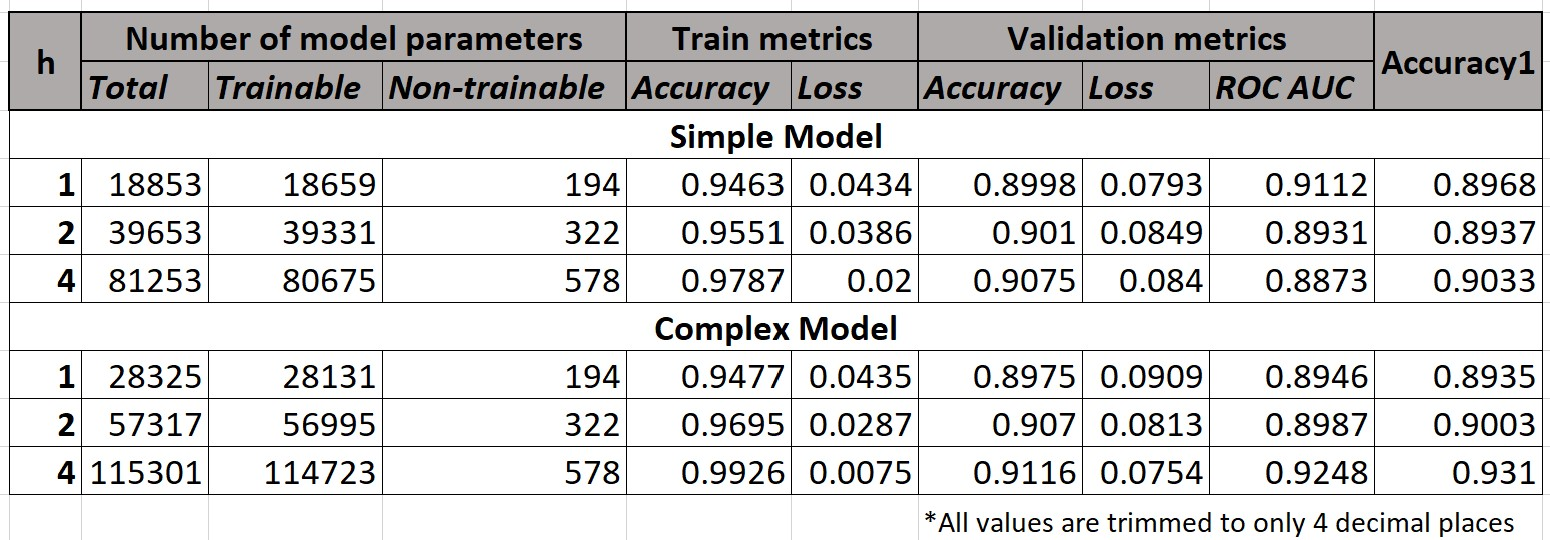
\includegraphics{res/img/table.jpg}
	
	For the explanation of what each column contains, look at section 5.3.

	\newpage
	
	\begin{enumerate}
		\item Simple model with $h = 1$.\\
		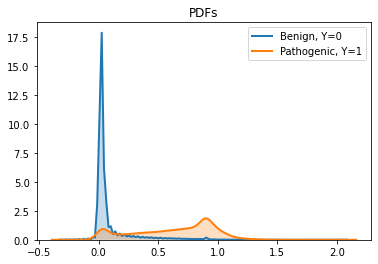
\includegraphics[scale=0.7]{res/img/s1pdf.png}\\
		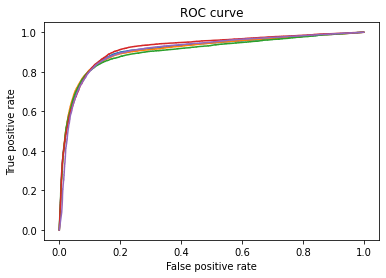
\includegraphics[scale=0.7]{res/img/s1roc.png}\\
		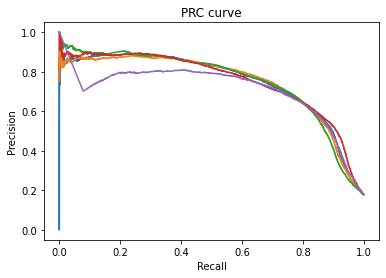
\includegraphics[scale=0.7]{res/img/s1prc.png}\\

		\item Simple model with $h = 2$.\\
		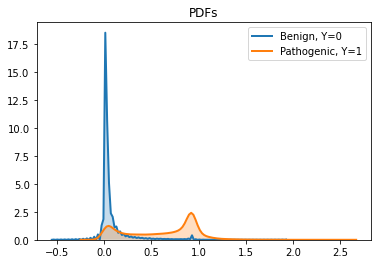
\includegraphics[scale=0.7]{res/img/s2pdf.png}\\
		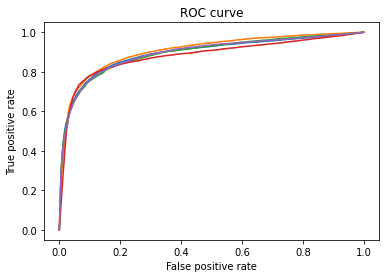
\includegraphics[scale=0.7]{res/img/s2roc.png}\\
		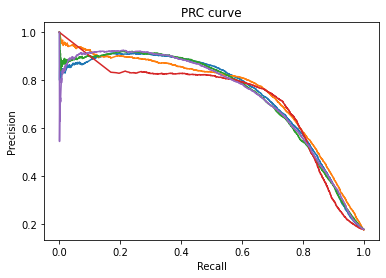
\includegraphics[scale=0.7]{res/img/s2prc.png}\\
		
		\item Simple model with $h = 4$.\\
		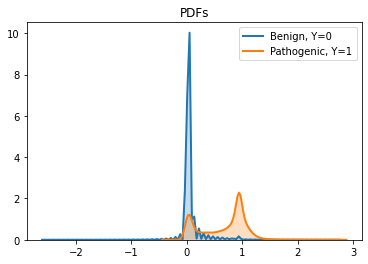
\includegraphics[scale=0.7]{res/img/s4pdf.png}\\
		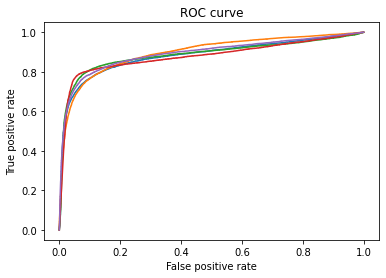
\includegraphics[scale=0.7]{res/img/s4roc.png}\\
		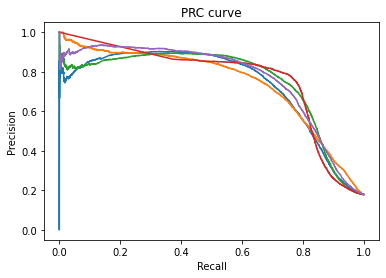
\includegraphics[scale=0.7]{res/img/s4prc.png}\\
		
		\item Complex model with $h = 1$.\\
		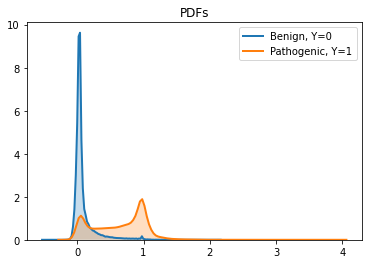
\includegraphics[scale=0.7]{res/img/c1pdf.png}\\
		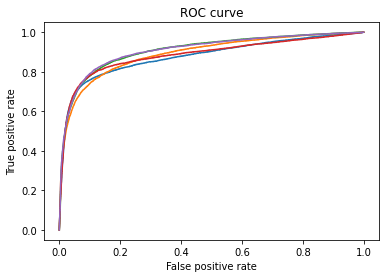
\includegraphics[scale=0.7]{res/img/c1roc.png}\\
		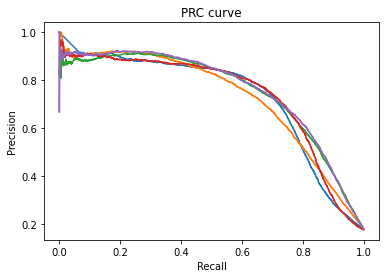
\includegraphics[scale=0.7]{res/img/c1prc.png}\\
		
		\item Complex model with $h = 2$.\\
		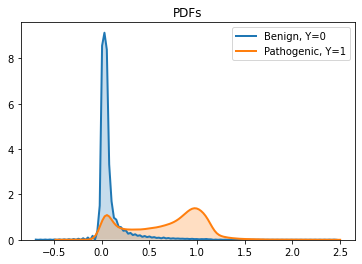
\includegraphics[scale=0.7]{res/img/c2pdf.png}\\
		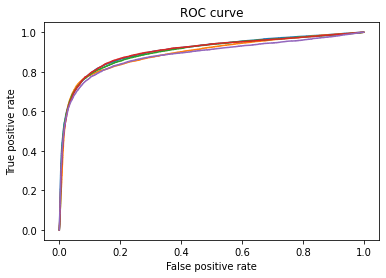
\includegraphics[scale=0.7]{res/img/c2roc.png}\\
		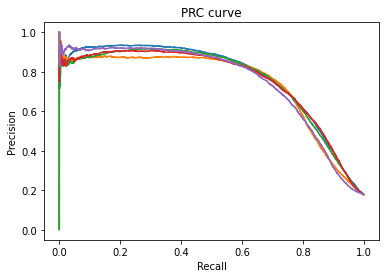
\includegraphics[scale=0.7]{res/img/c2prc.png}\\
		
		\item Complex model with $h = 4$.\\
		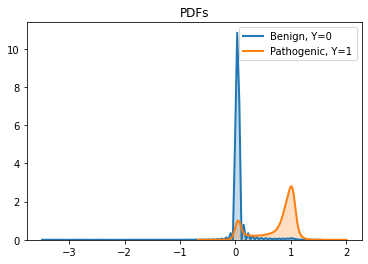
\includegraphics[scale=0.7]{res/img/c4pdf.png}\\
		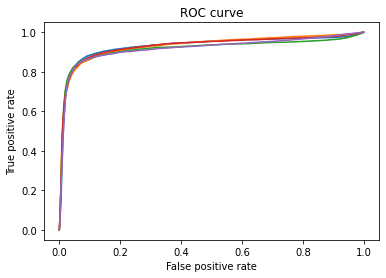
\includegraphics[scale=0.7]{res/img/c4roc.png}\\
		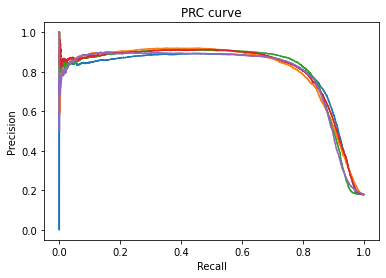
\includegraphics[scale=0.7]{res/img/c4prc.png}\\
		
	\end{enumerate}
	
	
	
	\section{Conclusions}
	\begin{enumerate}
		\item Almost all the metrics and the plots too indicate that the model gets better at the task of classification as the number of trainable parameters increase. Though there's an obvious limit to this, dependent upon the training examples.
		\item So, in conclusion the complex model with $h = 4$ performs the best, amongst all the tested ones, as per the metrics. It can also be verified from the pdf plots, the one for this model shows that it is able to separate the two classes in a better way as comapred to the other models.
		\item The validation accuracy of 91\% might seem great but it is actually not that great (because of the class imbalances), since the trivial classifier would give us an accuracy of 82\% by classifying all the mutations as benign. Though that's just focusing on the accuracy aspect, which is a grossly oversimplifies things, and there's much more to problems like these than just accuracy.
		\item It is also inferred from that results (and much more through the epoch vs accuracy plot for each fold of each model, which is shown in the notebook) that the validation accuracy struggles to go above 90\%, this is probably because the models are unable to learn all the complex patterns of the data. So, either the models need more information about the data which helps them easily classify the input, or they themselves need to be much more complex so that they're able to detect complex patterns in the data (but this approach would require much more data, since complex models would likely have more parameters to learn).
		\item It can be seen from the pdf that most of the loss in model accuracy is due to the model misclassifying some pathogenic mutations as benign. One would think that this would probably be because of the genes which have both benign and pathogenic mutations, but weirdly enough that is actually not the case. Accuracy1 is also reasonably good (compared to the train and validation accuracies), hence it is safe to say that the model performs (roughly) equally well (or poorly) on most genes.
		\item Some of the concepts learned and discussed in the class were also verified:
		\begin{enumerate}
			\item The PRC and ROC curves are indicative of how well a model performs.
			\item The PRC curve depends on the class priors, whereas ROC curve does not. This can be verified through the large deviations in PRC curves of some folds in the simple models, whereas all the ROC curves for that model are roughly the same.
			\item The rightmost point of the PRC curve is on the coordinates $(1, p(Y=1))$. Also that the curve may sometimes begin at $(0,0)$ and shoot straight up to $(0,1)$.
			\item Data cleaning, data preprocessing and evaluation are some really important (though not the most fun or interesting) aspects of practical machine learning. These things constituted more than 80\% of the time spent on this project.
		\end{enumerate}
	\item An interesting (but expected) observation is that the distributions actually look Gaussian (or a mixture of Gaussians).
	\item Another interesting observation made during the project, but it is actually not shown here, is that convolutional neural networks with 2-D (instead of 1-D) convolution layers were actually performing worse. This makes sense because even though we encode the data in 2-D matrices, it still essentially is a 1-D sequence of Amino Acids.
	\end{enumerate}
	
	
	\newpage
	
	\section{Individual Tasks}
	All the work was done by just one team member, since there were no others.
	
	
	
	\section{References}
	\begin{enumerate}
		\item https://www.nature.com/articles/s41588-018-0167-z
		\item https://gnomad.broadinstitute.org/
		\item https://ghr.nlm.nih.gov/primer
		\item https://www.uniprot.org/
		\item https://www.ncbi.nlm.nih.gov/clinvar/
		\item https://www.ebi.ac.uk/thornton-srv/databases/cgi-bin/DisaStr/GetPage.pl?varmap=TRUE
		\item https://en.wikipedia.org/
	\end{enumerate}
	
	

\end{document}